\chapter{Protokoły komunikacyjne (sieciowe)}
\label{r02}

W rozdziale tym przedstawiona zostanie architektura ISO/OSI stosu protokołów, dzięki którym wydajna i bezpieczna 
transmisja w sieci nie byłaby w ogóle możliwa: od protokołów TCP/IP, poprzez SSL do protokołów FTP i HTTP. 
Opisany zostanie także sposób identyfikacji i komunikacji urządzeń i zasobów sieciowych na różnych warstwach 
czyli DNS i URL. Najwięcej uwagi poświęcone zostanie na opis protokołu HTTP i sposób działania WWW.

\section{Wstęp}

Podstawow urządzenia komunikacyjne składają się z elementów, które przesyłają bity z jednego miejsca do drugiego. Jednakże
używanie ,,surowego'' sprzętu do komunikacji jest podobne do programowania przez wrowadzanie zer i jedynek -- jest to 
nieporęczne i niewygodne. Komputery podłączone do sieci są wyposażone w skomplikowane oprogramowanie udostępniejące
wygodny, wysokopoziomowy interfejs dla programów użytkownika. Oprogramowanie to obsługuje automatycznie większość 
niskopoziomowych szczegółów oraz problemów, co pozwala na łatwą komunikację między programami użytkowymi. W ten sposób
większość programów użytkownika przy komunikacji polega na oprogramowaniu sieciowym i nie komunikuje się bezpośrednio ze
sprzętem.

Wszystkie strony biorące udział w komunikacji muszą uzgodnić zbiór reguł używanych przy wymianie komunikatów. Zbiór reguł, 
które określają format komunikatów, oraz stosownych działań wymaganych dla każdego komunikatu nazywa się protokołem sieciowym.

\section{TCP/IP a ISO/OSI}

Aby sprawienie i efektywnie rozwiązać dowolne zadanie komunikacyjne oraz zaplanować zestaw 
protokołów stworzono model warstwowy \cite{siecikomputerowe}.
Zestaw protokołów można tym samym związać z określoną warstwą \cite{barylo1}.

Wcześnie w historii sieci \emph{International Organization for Stadarization} (ISO) opracowała model 7--warstwowy.
Model ISO/OSI jest standardem stanowiącym punkt odniesienia dla producentów oprogramowania i sprzętu sieciowego. 
Stosowanie się do zaleceń tego standardu zapewnić ma kompatybilność różnych produktów sieciowych, co implikuje 
możliwość swobodnego ich łączenia w tzw. system otwarty.
Wyróżnić w nim można: warstwę aplikacji, prezentacji i sesji -- nazywane warstwami górnymi, oraz
warstwę transportową, sieciową, łącza danych i fizyczną -- nazywane warstwami dolnymi. Warstwy górne zajmują się 
współpracą procesów wykonujących się w połączonych siecią komputerach. Warstwy dolne zapewniają prawidłową 
komunikację pomiędzy procesami. W każdej z warstw pracuje odpowiednie oprogramowanie realizujące funkcje 
protokołu danej warstwy. Protokoły poszczególnych warstw oferują określony rodzaj usług \cite{siecikomputerowe}:
\begin{description}
\item[warstwa aplikacji] -- określa sposób, w jaki dany program użytkowy korzysta z sieci np.: w wastwie tej działa protokół 
HTTP;
\item[warstwa prezentacji] -- protokoły tej warstwy określają jak prezentować dane. Takie protokoły są potrzebne gdyż różne
marki komputerów używają różnej wewnętrznej reprezentacji liczb i znaków -- protokoły tej warstwy tłumaczą reprezentację
na jednej maszynie na reprezentację na drugiej;
\item[warstwa sesji] -- odpowiedzialna jest za synchronizację danych przesyłanych pomiędzy aplikacjami, dzięki 
udostępnianym w tej warstwie tzw. punktom synchronizacji aplikacje są w stanie wzajemnie rozpoznać stan 
zaawansowania w przetwarzaniu wymienianych danych, umożliwia to wykrycie takich sytuacji jak np. spowodowane 
awarią zaprzestanie przetwarzania przez stowarzyszoną aplikację;
\item[warstwa transportowa] -- protokoły wastwy czwartej określają szczegóły obsługi połączenia -- są jednymi z najbardziej
skomplikowanych protokołów;
\item[warstwa sieciowa] --  protokoły tej warstwy określają sposób przyznawania adresów oraz przekazywania pakietów w sieci;
\item[warstwa łącza danych] -- protokoły tej warstwy określają sposób organizowania ramek i transmitowania ich przez sieć np.:
opis formatu ramki, rozpychania bitów lub bajtów oraz obliczania sum kontrolnych;
\item[warstwa  fizyczna] -- realizuje mechaniczne, elektryczne, funkcjonalne i proceduralne aspekty transmisji 
danych, czyli definiuje medium transmisyjne takie jak np. kabel miedziany.
\end{description}

Każda z warstw udostępnia warstwie bezpośrednio wyższej zestaw funkcji realizujących  zadania danej warstwy i 
korzysta z zestawu funkcji udostępnianych przez warstwę bezpośrednio niższą. Nie jest możliwe by np. warstwa 
transportowa korzystała z funkcji warstwy łącza danych z pominięciem warstwy sieciowej. Porcję danych 
przeznaczonych do wysłania nazywa się pakietem. Wysyłany pakiet musi przejść kolejno przez wszystkie warstwy 
modelu ISO/OSI od warstwy aplikacji do warstwy fizycznej. W trakcie tej wędrówki pakiet obrasta w informacje 
kontrolne umożliwiające protokołowi danej warstwy zarządzanie danymi i połączeniami, tę informację kontrolną 
nazywamy nagłówkiem lub końcówką w zależności od tego, czy jest dodawana na początku, czy na końcu danych. 
Nagłówek warstwy wyższej traktowany jest w warstwie niższej jako część danych i nie podlega tam żadnym zmianom. 
Pakiet odbierany odbywa drogę odwrotną -- od warstwy fizycznej do warstwy aplikacji. W trakcie tej drogi 
protokoły poszczególnych warstw usuwają swoje nagłówki, tak aby do aplikacji docelowej pakiet dotarł w takiej 
postaci, w jakiej został wysłany. Poniższy rysunek schematycznie przedstawia opisany proces.
\begin{figure}[h]
\centering
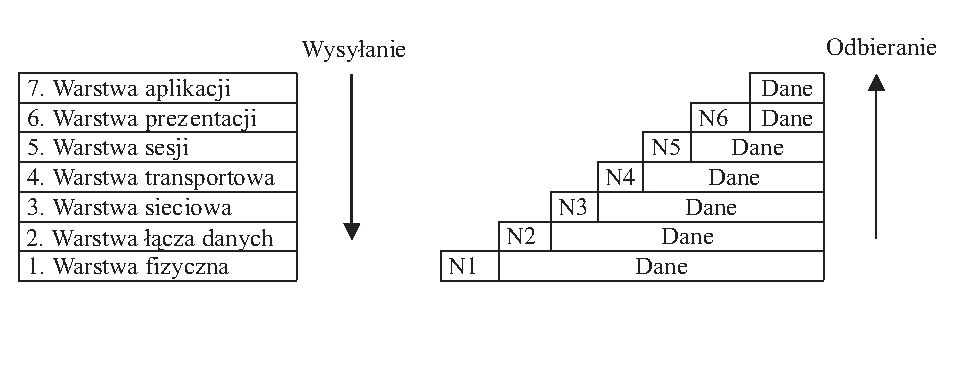
\includegraphics[width=5in]{./rysunki/nadawanie_i_odbieranie_naglowkow.eps}
\caption{Proces nadawania i odbierania nagłówków transmitowanym danym}
\label{nadawanie}
\end{figure}

Protokoły poszczególnych warstw zarządzają danymi w specyficzny dla siebie sposób, mogą np. dokonać segmentacji, 
czyli podziału danych na mniejsze fragmenty przed przesłaniem ich do niższej warstwy. Każdy fragment otrzymuje 
wtedy odpowiedni nagłówek, który umożliwia analogicznemu protokołowi w komputerze adresata danych scalenie 
fragmentów podczas odbierania pakietu. Nagłówki umożliwiają również zarządzanie połączeniami np. 
multipleksowanie połączeń czyli wykorzystywanie jednego połączenia, ściślej -- punktu dostarczania usług SAP 
(ang. \emph{Service Access Point})  warstwy niższej, np. sieciowej do obsługi kilku połączeń nawiązanych w warstwie 
bezpośrednio wyższej (tu transportowej). Odpowiednia informacja zawarta w nagłówku warstwy wyższej umożliwia 
wtedy identyfikację odbiorcy danych. Model ISO/OSI definiuje dwa tryby komunikacji. Komunikacje połączeniową 
stosuje się gdy kluczowym wymaganiem jest niezawodność transmisji, musi być wtedy znany zarówno odbiorca jak i 
nadawca danych, a odbiorca potwierdza dotarcie do niego każdego fragmentu pakietu lub sygnalizuje konieczność 
retransmisji w przypadku błędu. Komunikacja bezpołączeniowa nie zapewnia niezawodności, dane wysyła się bez 
oczekiwania na potwierdzenie, a nadawca  i odbiorca nie są znani, chyba że wynika to z zawartości pakietu, 
pakiety wysyłane w trybie bezpołączeniowym nazywamy datagramami.

W praktyce nie istnieje rozwiązanie przemysłowe, które ściśle implementowałoby wszystkie warstwy modelu ISO/OSI, 
częstą praktyką jest np. łączenie warstw fizycznej i łącza danych w jedną warstwę. Również protokoły TCP/IP nie 
są w pełni kompatybilne z modelem ISO/OSI, nie są też jednak całkowicie niekompatybilne. Wzajemną relację 
architektury ISO/OSI i TCP/IP przedstawia poniższy rysunek \cite{barylo1}.
\begin{figure}[h]
\centering
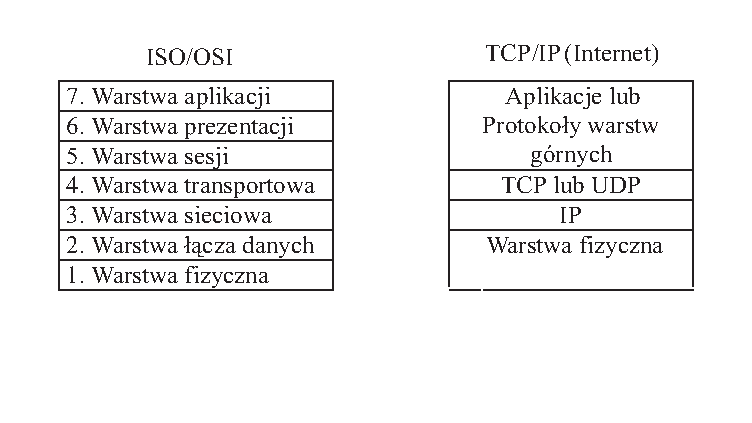
\includegraphics[width=5in]{./rysunki/architektura_ISO_a_tcp.eps}
\caption{Architektura ISO/OSI a TCP/IP}
\label{ISO_TCP}
\end{figure}
\section{Protokół IP}

Protokół IP (ang. \emph{Internet Protocol}) działa w warstwie sieciowej i jest podstawowym protokołem rodziny TCP/IP --
wszystkie dane napływające z wyższych warstw przesyłane są w sieci jako datagramy IP. Protokół ten świadczy 
zawodne, bezpołączeniowe usługi dostarczania pakietów. Przez zawodne rozumiemy tu taką właściwość, że IP nie 
daje gwarancji dostarczenia pakietu do punktu przeznaczenia, a wszelkie mechanizmy zapewnienia niezawodności transmisji muszą
zostać zapewnione przez protokoły wyższych warstw (np. TCP). Termin bezpołączeniowy oznacza tu, że IP nie 
przechowuje żadnej informacji na temat prawidłowo przesyłanych datagramów, każdy z nich obsługiwany jest osobno, 
co w praktyce może oznaczać, że datagramy mogą docierać do adresata w innej kolejności, niż zostały wysłane. 
Wszystkie dane konieczne do poprawnej pracy IP zawarte są w jego nagłówku, który typowo (jeśli nie zawiera 
opcji) ma długość 20 bajtów i przedstawiony poniżej format \cite{barylo2}.

\begin{figure}[h]
\centering
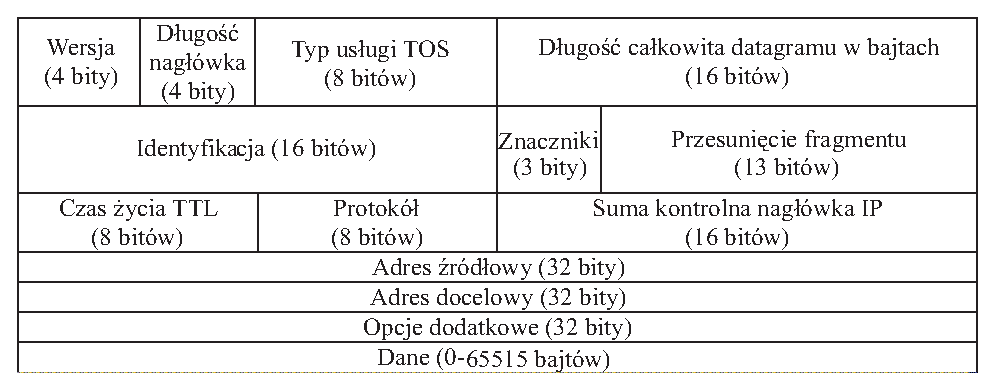
\includegraphics[width=5in]{./rysunki/datagram_ip.eps}
\caption{Format datagramu IP z wyróżnieniem nagłówka}
\label{datagram_ip}
\end{figure}

Pole \emph{długość nagłówka} określa długość nagłówka w 32--bitowych słowach i wraz z polem Długość całkowita datagramu 
służy do określenia miejsca w którym zaczynają się właściwe dane. Całkowita długość datagramu ograniczona jest 
zwykle przez warstwę fizyczną np. dla sieci Ethernet jest to maksymalnie 1500 bajtów a wielkość tę nazywamy MTU 
(ang. \emph{Maximum Transmission Unit}) danej sieci.

Pole \emph{identyfikacja} zawiera unikalny numer dla każdego wysyłanego datagramu. Jeżeli przechodząc przez kolejne 
węzły sieci datagram musi zostać podzielony, to wartość ta jest kopiowana do wszystkich nagłówków IP 
powstających fragmentów i wraz z wartością pola Przesunięcie fragmentu umożliwia poprawne scalenie datagramu w 
punkcie docelowym. Pomocne są w tym również wartości bitów pola Znaczniki. Ustawienie jednego z nich wskazuje, 
że istnieje kilka fragmentów datagramu, ustawienie drugiego zabrania fragmentacji datagramu.

Pole \emph{czas życia TTL} wyznacza  maksymalną liczbę routerów przez które może przejść datagram (routerem 
nazywamy tu specjalizowane urządzenie lub odpowiednio oprogramowany komputer służące do przekazywania datagramów 
pomiędzy sieciami różniącymi się w warstwie fizycznej np. Ethernet i Token Ring, lecz pracującymi w oparciu o 
wspólny protokół warstwy sieciowej - IP). Wartość tego pola jest wielkością całkowitą zmniejszaną o jeden przez 
każdy router, do którego dociera datagram. Datagram z wartością TTL równą 0 usuwany jest z sieci, co zapobiega 
krążeniu w niej błędnie zaadresowanych datagramów.

Pole \emph{protokół} określa typ protokołu będącego nadawcą datagramu i jednocześnie protokół który powinien 
odebrać datagram w punkcie docelowym.

Kluczowe znaczenie dla wyznaczania trasy przesyłania datagramu mają pola \emph{adres docelowy} i \emph{adres źródłowy}. Na 
podstawie wartości pola Adres docelowy protokół IP dynamicznie wyznacza kolejny węzeł sieci na drodze pakietu, 
proces ten nazywamy marszrutowaniem IP. Adres IP jest 32--bitowym numerem, który w sposób unikalny wyznacza 
miejsce podłączenia interfejsu sieciowego (karty sieciowej) do sieci. W adresie IP wyróżniamy część globalną 
określającą adres sieci i część lokalną identyfikującą komputer w konkretnej sieci. Istnieje pięć klas adresów IP (Rys.: \ref{klasy_ip}):
\begin{figure}[h]
\centering
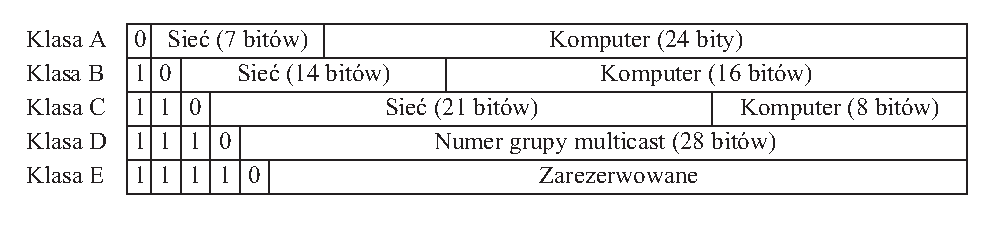
\includegraphics[width=5in]{./rysunki/klasy_adresow.eps}
\caption{Klasy adresów IP}
\label{klasy_ip}
\end{figure}

Aby zapewnić unikalność adresów sieci przydzielane są one centralnie przez organizację InterNIC. Adres zapisuje
się zwykle w tzw. notacji kropkowo -- dziesiętnej, dzieli się go na cztery ośmiobitowe  grupy i wartość każdej z 
nich zapisuje dziesiętnie np.156.17.130.10 jest adresem serwera pocztowego Instytutu Sterowania i Techniki Systemów
Politechniki Wrocławskiej.

Istnieją trzy typy adresów IP: adres unicast dotyczy pojedynczego komputera, adres broadcast dotyczy 
wszystkich komputerów w danej sieci a adres multicast obejmuje grupę komputerów należących do jednej grupy 
multicastowej. Obecnie wszystkie implementacje IP muszą obsługiwać tzw. adresowanie podsieci. Zamiast traktować 
adres IP jako proste złożenie adresu sieci i hosta (komputera) w części adresu wskazującej hosta wydziela się 
adres podsieci i właściwy adres hosta. Wynika to z faktu, że adresy klasy A i B przeznaczają zbyt wiele bitów na 
adres hosta, adres klasy B umożliwia np. zaadresowanie 65535 komputerów, a rzadko spotyka się tak wiele hostów 
podłączonych do jednej sieci. Podział 16 bitowego adresu hosta klasy B na dwie części ośmiobitowe umożliwia 
utworzenie w jednej sieci 255 podsieci z 254 hostami w każdej z nich. Decyzję o podziale na podsieci podejmuje 
lokalny administrator, a informację o tym jaka ilość bitów przeznaczona jest na adres podsieci przechowywana 
jest przez tzw. maskę podsieci. Jest to wartość 32--bitowa  zawierająca jedynki dla części adresującej sieć i 
podsieć oraz zera dla części adresującej hosta. Maska podsieci ma w omówionym przypadku postać 255.255.255.224.

Istnieje kilka zarezerwowanych adresów IP wykorzystywanych do celów specjalnych. Obowiązkowym adresem 
specjalnym jest adres interfejsu pętli zwrotnej (ang. \emph{loopback}). Większość systemów przypisuje temu interfejsowi 
z definicji adres 127.0.0.1, choć poprawny jest dowolny adres klasy A z adresem sieci 127. Datagramy kierowane 
na adres pętli zwrotnej przechodzą przez warstwę transportową i sieciową po czym są zawracane w górę stosu 
TCP/IP. Najczęstszym zastosowaniem pętli zwrotnej jest testowanie poprawności działania protokołów TCP/IP. 
Niektóre systemy (np. system AIX) umożliwiają dodawanie aliasów (dodatkowych adresów) do adresu interfejsu pętli 
zwrotnej.

Każdy komputer (host) podłączony do sieci IP posiada co najmniej jeden adres IP, hosty posiadające kilka 
interfejsów sieciowych posiadają po jednym adresie dla każdego interfejsu. Wszystkie te adresy, wraz z adresami 
specjalnymi i adresami typu broadcast przechowywane są w tzw. tablicy marszrutowania (routingu). Protokół IP po otrzymaniu 
datagramu sprawdza, czy jego adres IP zgodny jest z którymś z adresów hosta lub jednym z adresów specjalnych. 
Jeśli tak jest datagram zostaje zaakceptowany. Postępowanie w przeciwnym wypadku zależy od tego, czy warstwa IP 
skonfigurowana jest jako router. Jeżeli host nie jest routerem następuje odrzucenie datagramu, w przeciwnym wypadku
uruchamiany jest opisany poniżej algorytm marszrutowania.

Marszrutowanie IP dokonywane jest na podstawie kolejnych przejść pomiędzy węzłami sieci zapisanych (wraz z 
adresami własnymi hosta) w tablicy marszrutowania. Pojedynczy rekord tablicy routingu zawiera znany adres 
docelowy IP i adres IP na który należy skierować datagram jeśli jego adres docelowy jest zgodny z adresem 
zapisanym w rekordzie. Jeżeli nadawca i odbiorca są bezpośrednio połączeni rekord tablicy marszrutowania zawiera 
wskazanie (w postaci adresu IP) na adresata datagramu, o czym informuje specjalny znacznik w danym rekordzie. 
W przeciwnym wypadku jest to adres routera stanowiącego połączenie z inną siecią lokalną lub punkt wyjścia do 
sieci rozległej. Zakłada się że router taki znajduje się bliżej punktu docelowego datagramu, gdyż IP nie zna 
pełnej trasy dla żadnego z datagramów adresowanych poza sieć lokalną. Wybór drogi datagramu przebiega 
następująco \cite{barylo2}: 
w pierwszej kolejności poszukiwany jest rekord zawierający w pełni zgodny adres docelowy IP. Jeśli zostanie on 
znaleziony, datagram jest wysyłany na adres wskazany przez rekord. Może być to adres docelowy lub znane 
przejście przez router do innej sieci lokalnej.
Następnie w tablicy marszrutowania  poszukiwany jest rekord z adresem sieci zgodnym z adresem sieci 
marszroutowanego datagramu. Jeśli poszukiwania zakończą się sukcesem datagram jest wysyłany na zawarty tam adres. 
W ten sposób mogą być obsługiwane  datagramy zaadresowane do hostów połączonych z nadawcą przez wspólną sieć 
(w sensie zgodności adresów globalnych IP). 
W przypadku niepowodzenia poprzednich poszukiwań datagram wysyłany jest na adres IP routera domyślnego.

Ostatnią czynnością dokonywaną zanim datagram rzeczywiście opuści komputer nadawcy jest ustalenie jego adresu 
fizycznego w danej sieci lokalnej (np. adresu Ethernet lub Token Ring). Każde urządzenie: komputer, router, czy 
most (bridge) posiada unikalny w obszarze danej sieci lokalnej adres fizyczny. Odwzorowanie adresu IP w adres fizyczny 
dokonuje się przy użyciu protokołu ARP (ang. \emph{Address Resolution Protocol}), opis jego działania leży poza 
zakresem tej pracy.
Wypada zaznaczyć, że adresy IP klasy B wyczerpały się w roku 1997, co wymusiło wprowadzenie nowej specyfikacji
protokołu IP tzw. IPv6, który wprowadza adresy 128 bitowe. 

\section{Protokół TCP}

Protokół TCP (ang. \emph{Transmission Control Protocol}) zapewnia niezawodne, zorientowane 
połączeniowo, oparte na strumieniach bajtów (tzn. nie stosujące żadnego arbitralnego podziału przesyłanych 
danych na jednostki stałej długości) usługi warstwy transportowej. Przed rozpoczęciem transmisji dwie aplikacje 
używające TCP muszą ustanowić połączenie w postaci wirtualnego kanału transmisyjnego. Niezawodność tego 
połączenia zapewniana jest przez działania takie jak: podział przesyłanych danych na segmenty o rozmiarze 
optymalnym ze względu na poprawność transmisji; utrzymywanie dla każdego segmentu osobnego zestawu zegarów 
wyznaczających m. in. maksymalny czas oczekiwania na potwierdzenie odbioru segmentu i wymuszającego retransmisję 
w przypadku przekroczenia tego czasu; używanie obowiązkowych sum kontrolnych; odrzucanie zdublowanych 
datagramów IP; zdolność rozpoznania kolejności datagramów IP (mogą one docierać w kolejności innej niż były 
wysyłane).

Informację kontrolną segmentu TCP zawiera przedstawiony poniżej nagłówek \cite{barylo2}.
\begin{figure}[h]
\centering
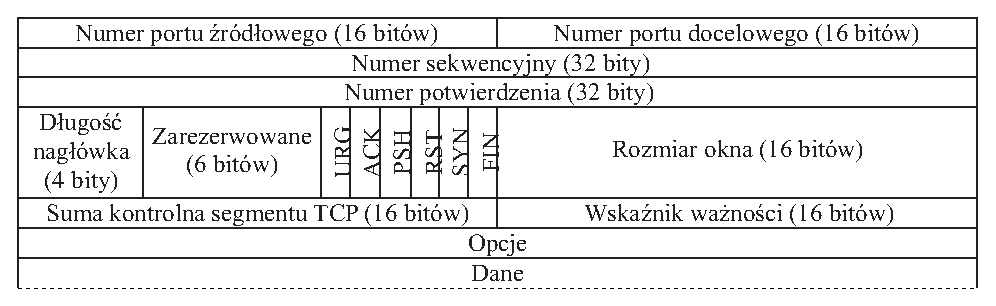
\includegraphics[width=5in]{./rysunki/format_segmentu_tcp.eps}
\caption{Format segmentu TCP z wyróżnieniem nagłówka.}
\label{segment_TCP}
\end{figure}

Pola \emph{numer portu źródłowego} i \emph{numer portu docelowego} zawierają wielkości całkowite i pełnią kluczową rolę w 
identyfikacji połączeń TCP. Numery portów od 1 do 1023 są zarezerwowane dla tzw. usług dobrze znanych i 
zazwyczaj przydzielane są aplikacjom pracującym jako serwery. Przykładowo serwery WWW (protokół HTTP) otrzymują 
numer portu 80, serwery FTP wykorzystują porty 20 i 21 a serwery pocztowe (SMTP) port 25. Do nawiązania 
połączenia proces klienta (np. przeglądarka WWW) uzyskuje od protokołu TCP tzw. numer krótkotrwały unikalny dla 
każdej aplikacji używającej TCP w danym hoście. W przypadku przeglądarki WWW może być to numer 80 lub dowolny 
numer z zakresu 1024... 5000. Para port źródłowy -- port docelowy jest wystarczająca do identyfikacji połączenia 
po stronie klienta. Jeśli nawet użytkownik uruchomi dwie identyczne aplikacje (np. dwie przeglądarki WWW), to 
otrzymają one różne numery krótkotrwałe. Po stronie serwera sytuacja jest trudniejsza, typowo serwer poprzez 
multipleksację portu obsługuje wiele połączeń z użyciem jednego numeru portu źródłowego (np. 80 dla serwera WWW),
może się więc zdarzyć, że dwóch niezależnych klientów zgłosi ten sam numer krótkotrwały portu docelowego. Do 
jednoznacznej identyfikacji połączeń wykorzystuje się kombinację numeru portu i adresu IP nazywaną gniazdem. 
Gniazda są jednym z podstawowych pojęć interfejsu programisty TCP/IP.

Jak już wspomniano TCP przesyła dane w postaci strumienia bajtów, w praktyce oznacza to, że wysyłany 
segment danych może mieć każdorazowo inną  długość. Do umożliwienia uformowania z segmentów oryginalnego pakietu 
służy wartość pola \emph{numer sekwencyjny}. Jeśli rozpatrzymy strumień bajtów przesyłany tylko w jedną stronę, to 
wartość tego pola określa  numer jaki ma w strumieniu ostatni bajt segmentu. Wartość początkową numeru 
sekwencyjnego ustala nadawca w momencie ustanawiania połączenia. Jeśli początkowym numerem sekwencyjnym było 
100, a pierwszy segment ma długość 1024 bajty, to jego numerem sekwencyjnym jest 1123. Pierwszy bajt kolejnego 
segmentu składającego się na pakiet będzie miał numer 1124, jeśli segment ten ma długość 125 bajtów, to jego 
numerem sekwencyjnym jest 1248. Koniec strumienia oznacza się przez ustawienie flagi bitowej FIN w nagłówku 
ostatniego segmentu.

TCP wymaga potwierdzeń odbioru każdego przesłanego segmentu. Służy do tego pole \emph{numer potwierdzenia}. Jeśli 
znów rozpatrywać przesyłanie danych w jedną tylko stronę, to po odebraniu segmentu o numerze sekwencyjnym 1123 
klient wysyła (pozbawiony danych) segment TCP z ustawioną flagą bitową ACK i wartością numeru potwierdzenia 1124 
(jest to numer kolejny oczekiwanego bajtu). Aby zapewnić niezależne przesyłanie danych w obydwu kierunkach, 
każda ze stron pamięta numery sekwencyjne wymienianych segmentów. Opisany powyżej segment potwierdzenia posiada 
więc ustalany przez jego nadawcę numer sekwencyjny (np. 136), który serwer musi potwierdzić ustawiając flagę ACK 
i umieszczając w polu Numer sekwencyjny odpowiednią wartość (tutaj 137). Konsekwencją takiej strategii wymiany 
potwierdzeń jest fakt, że w trakcie wymiany danych flaga ACK jest ciągle ustawiona (ma wartość logiczną 1).
Pole Długość nagłówka zawiera liczbę 32--bitowych słów składających się na nagłówek, następuje po nim 6 
zarezerwowanych bitów i kolejno 6 flag bitowych. Istotną flagą jest SYN, która jest ustawiona podczas wymiany 
segmentów nawiązujących połączenie i ustalania początkowych numerów sekwencyjnych. 

Pole \emph{rozmiar okna} zawiera wartość całkowitą, przy pomocy której odbiorca deklaruje jaką ilość bajtów 
nadawca może wysłać bez oczekiwania na potwierdzenie (inaczej -- jaką ilość bajtów odbiorca jest w stanie przyjąć 
jednorazowo). Pole ma zastosowanie w przypadku transmisji wg tzw. protokołu przesuwnego okna, a jego wartość 
może się zmieniać w trakcie  transmisji.

Ważną rolę w trakcie nawiązywania połączenia pełni pole \emph{opcje}. W polu tym uczestnicy połączenia wymieniają 
się informacją jak duży jest pojedynczy segment, który są w stanie przyjąć. Ustalone w ten sposób maksymalne 
wielkości segmentu MSS (ang. \emph{Maximum Segment Size}) pozostają stałe dla obydwu końcówek połączenia przez cały 
czas jego trwania. 

Wartość tę ustala się z uwzględnieniem nakładanego przez warstwę fizyczną ograniczenia na maksymalny rozmiar 
datagramu IP (MTU).

Aby móc zarządzać połączeniami oprogramowanie protokołu TCP utrzymuje tablicę połączeń. Pojedynczy rekord takiej 
tablicy opisuje jedno połączenie i zawiera pola: 
\begin{itemize}
\item Status (zamknięte, w trakcie zamykania, oczekiwanie na potwierdzenie itp.)
\item Adres lokalny -- adres IP hosta źródłowego (przechowującego tablicę)
\item Port lokalny -- numer portu hosta źródłowego
\item Adres zdalny -- adres IP hosta docelowego
\item Port zdalny -- numer portu docelowego
\end{itemize}

Protokół TCP wykorzystywany jest przez wiele protokołów wyższych warstw, dla których najistotniejszą sprawą jest 
zapewnienie niezawodności transmisji. TCP używają m. in. HTTP, FTP czy SMTP, które zostaną krótko omówione w 
dalszej części tej pracy. System DNS korzysta z protokołu TCP podczas wymiany danych pomiędzy serwerami DNS w 
trakcie uaktualniania ich tablic odwzorowań.

\section{Protokół UDP}

Protokół UDP (ang. \emph{User Datagram Protocol}) jest prostym, bezpołączeniowym protokołem warstwy transportowej 
wykorzystującym datagramy. Z każdego pakietu danych skierowanego do UDP przez warstwy górne formowany jest 
jeden datagram UDP, z którego (inaczej niż w przypadku TCP) tworzony jest dokładnie jeden datagram IP. Aplikacja 
wysyłająca pakiet musi sama zadbać o to, by jego długość nie przekroczyła MTU. UDP (w przeciwieństwie do TCP) 
nie implementuje żadnych mechanizmów zapewniających niezawodność transmisji.  Nagłówek datagramu UDP ma bardzo 
prosty format \cite{barylo2}.
\begin{figure}[h]
\centering
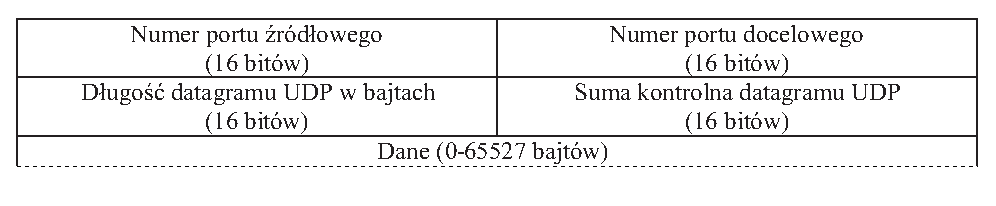
\includegraphics[width=5in]{./rysunki/datagram_udp.eps}
\caption{Datagram UDP z wyróżnionym nagłówkiem.}
\label{datagram_udp}
\end{figure}
 
\section{Protokół FTP}

Protokół FTP (ang. \emph{File Transfer Protocol}) jest standardowym w Internecie protokołem przesyłania dowolnego 
rodzaju plików. Jest to protokół warstw wyższych, i przez to jest często błędnie utożsamiany z aplikacjami 
klienta FTP. FTP korzysta w warstwie transportowej z usług protokołu TCP. Do obsługi transmisji FTP, w 
przeciwieństwie do większości protokołów, otwiera aż dwa połączenia TCP : połączenie sterujące o numerze portu 
docelowego 21 i połączenie transmisji danych o numerze portu 20. Przez połączenie sterujące aplikacje FTP 
wymieniają zdefiniowane w protokole polecenia i potwierdzenia. Połączenie transmisji używane jest do binarnego 
przesyłania danych. Schemat obsługi połączenia przez procesy klienta i serwera FTP przedstawia rysunek \ref{polaczenie_ftp}.
\begin{figure}[h]
\centering
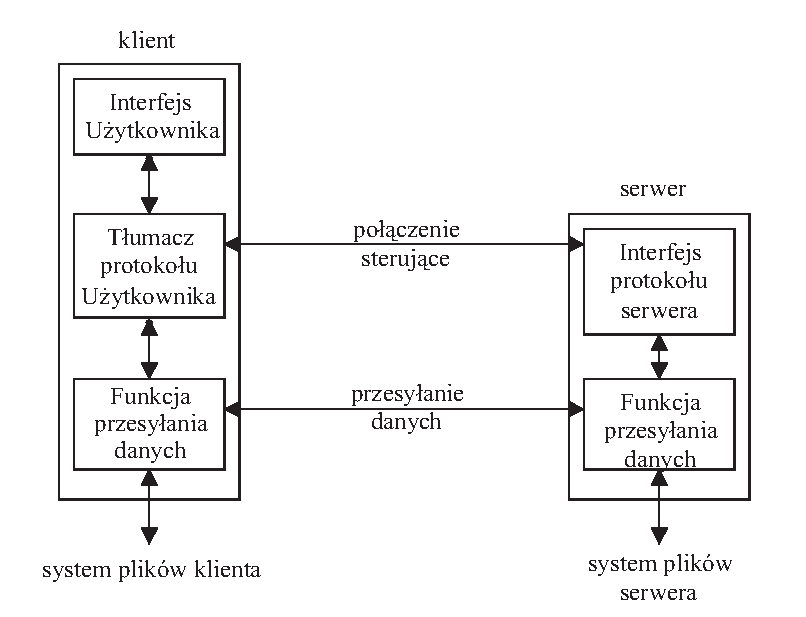
\includegraphics[width=5in]{./rysunki/obsluga_ftp.eps}
\caption{Obsługa połączenia ftp.}
\label{polaczenie_ftp}
\end{figure}

Połączenie przesyłania danych nawiązywane jest dla każdego przesyłanego pliku. FTP może przesyłać pliki w 
jednym z trzech trybów: jako strumień bajtów, jako serię bloków podzielonych nagłówkami lub w rzadko stosowanym 
trybie z kompresją FTP (kompresji podlegają tylko ciągi zerowych bajtów). FTP rozpoznaje formaty ASCII i EBCDIC 
-- przesyłane są one w postaci rekordów o stałej długości, pozostałe pliki traktowane są jako pliki binarne i 
przesyłane jako strumień bajtów.

Polecenia FTP wymieniane przez połączenie sterujące mają postać ciągów wielkich liter ASCII o długości 3 
lub 4 bajtów. Każde nawiązanie połączenia z serwerem FTP wymaga podania nazwy użytkownika i hasła, jest to 
prosty mechanizm zapewniający kontrolę dostępu do zasobów serwera. O tym, jakie pliki udostępniać konkretnym 
użytkownikom decyduje administrator serwera FTP.
Według badań prowadzonych w szkieletowej sieci NSFNET dane FTP stale stanowią ok. 20\% pakietów 
transmitowanych w tej sieci. 

\section{Protokół SNMP}

Protokół SNMP (ang. \emph{Simple Network Management Protocol}) pierwotnie zaprojektowano jako uniwersalne narzędzie, 
które umożliwi zdalne nadzorowanie śluz (ang. \emph{gateway})  i routerów w sieciach rozległych. W miarę jego rozwoju 
protokół uzupełniono o możliwość zarządzania wszelkim typem urządzeń sieciowych w sieciach TCP/IP. SNMP każdej 
sieci opiera się o trzy składniki:
\begin{itemize}
\item MIB (ang. \emph{Management Information Base}) jest to baza danych opisująca stan danego urządzenia;
\item SMI (ang. \emph{Structure and Identification of Management Information}) jest zestawem powszechnie stosowanych 
schematów służących odwoływaniu się do zmiennych MIB;
\item SNMP określa zasady komunikowania się pomiędzy aplikacją zarządzającą siecią (serwerem SNMP), a procesem 
sterującym urządzeniem (agentem).
\end{itemize}

Każdy element sieci, który ma być zarządzany przez SNMP, musi przechowywać informację o parametrach określających
stan danego elementu, a mających wpływ na pracę sieci. Baza danych zawierająca te parametry to właśnie MIB. W 
przypadku urządzenia takiego jak router rekord MIB może np. zawierać informację o stopniu zapełnienia jego 
buforów pamięci. MIB nie musi dotyczyć elementów ściśle sprzętowych istnieją np. MIB systemów operacyjnych. 
Sposób odwoływania się do elementów MIB określają schematy SMI.

W każdej sieci, której elementy zarządzane są według standardów SNMP istnieje wydzielony host, na którym 
pracuje specjalistyczna aplikacja (serwer SNMP) służąca monitorowaniu i zarządzaniu pracą sieci. Proces, który 
działa w zarządzanym elemencie i  aktualizuje MIB oraz udostępnia serwerowi jej zmienne lub ustawia je na zadane 
przez serwer wartości nazywany jest agentem SNMP.

W celu umożliwienia komunikacji pomiędzy serwerem a agentami SNMP definiuje pięć typów komunikatów. Trzy 
z nich wysyłane są zawsze w kierunku serwer--klient i służą pobieraniu lub ustawianiu zmiennych MIB. Dwa typy 
komunikatów wysyłane są w kierunku klient--serwer. Jeden z nich zwraca żądaną lub nowo ustawioną wartość 
zmiennej MIB, drugi jest komunikatem alarmowym wysyłanym przez agenta w przypadku błędnej pracy urządzenia lub 
przekroczenia krytycznej wartości przez którąś ze zmiennych MIB.
Serwer SNMP musi utrzymywać w miarę aktualną informację o stanie sieci, dlatego agenci SNMP przepytywani 
są w regularnych odstępach czasu, posiadając jednocześnie możliwość raportowania o sytuacjach awaryjnych. Fakt, 
że cztery z pięciu możliwych rodzajów komunikacji pomiędzy serwerem a agentem SNMP to pary typu pojedyncze 
pytanie--pojedyncza odpowiedź (wyjątek stanowią komunikaty alarmowe) oraz chęć minimalizacji obciążenia sieci 
powodowanego przez pakiety służące jej zarządzaniu spowodowały, że SNMP w warstwie transportowej korzysta z 
usług UDP. Zawodność tego protokołu sprawia, że serwery SNMP powinny (szczególnie w sytuacjach awaryjnych) 
stosować mechanizmy odmierzania czasu na odpowiedź agenta i ewentualnej retransmisji komunikatów. Warto dodać, 
że SNMP nie jest zależny w warstwie sieciowej od IP, przy odpowiedniej konfiguracji rolę protokołu sieciowego 
może spełniać np. IPX/SPX.

\section{Protokół SMTP}

Protokół SMTP (ang. \emph{Simple Mail Transfer Protocol}) jest prostym protokołem warstw górnych wykorzystywanym do 
przesyłania poczty elektronicznej w sieciach TCP/IP. W warstwie transportowej SMTP wykorzystuje protokół TCP i 
posiada przydzielony numer portu 25. Należy wyjaśnić, że programy pocztowe, z którymi kontaktują się szeregowi 
użytkownicy Internetu stanowią jedynie końcowe narzędzia, w terminologii fachowej nazywane agentami użytkownika 
UA (ang. \emph{User Agent}) służące do pobierania listów z elektronicznych skrzynek pocztowych lub umieszczania ich w 
kolejce do najbliższego serwera pocztowego. Programy rzeczywiście zajmujące się przesyłaniem wiadomości pomiędzy 
serwerami pocztowymi nazywane są agentami przesyłania komunikatów MTA (ang. \emph{Message Transfer Agent}). Przykładem 
MTA jest unixowy Sendmail. Protokół SMTP służy właśnie do komunikacji pomiędzy poszczególnymi MTA. Schemat 
przesyłania poczty w Internecie przedstawia poniższy rysunek.
\begin{figure}[h]
\centering
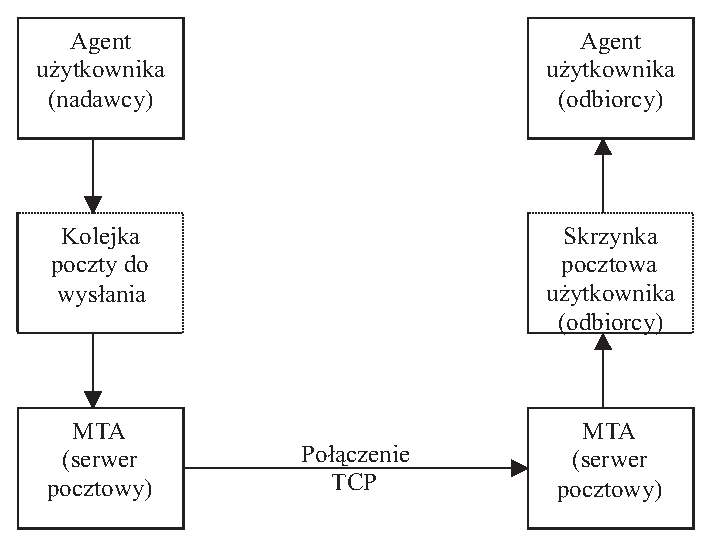
\includegraphics[width=5in]{./rysunki/obsluga_poczty.eps}
\caption{Schemat przesyłania poczty elektronicznej}
\label{poczta}
\end{figure}

Komunikacja pomiędzy MTA odbywa się według modelu klient -- serwer, przy czym klientem nazywamy MTA, który inicjuje dane 
połączenie. Połączenie rozpoczyna się od przesłania danych identyfikujących nadawcę, a w odpowiedzi nadchodzi pakiet 
identyfikujący odbiorcę. Następnie przesyłana jest właściwa wiadomość i połączenie jest zamykane. Do obsługi poczty 
elektronicznej SMTP definiuje tylko 13 poleceń (dla porównania FTP posiada 40 poleceń), które są czterobajtowymi ciągami 
wielkich liter ASCII.

Wiadomość elektroniczna składa się w SMTP z trzech części. Koperty czyli danych pozwalających MTA zidentyfikować 
nadawcę i odbiorcę wiadomości, nagłówków czyli danych wykorzystywanych przez agentów użytkownika (np. data 
wysłania wiadomości) i właściwej wiadomości.
Pakiety SMTP stanowią od 8 do 13 procent pakietów transmitowanych w sieci szkieletowej NSFNET. 

\section{Protokół POP3.}

Opisany powyżej protokół SMTP jest efektywnym narzędziem umożliwiającym przesyłanie poczty elektronicznej 
pomiędzy pracującymi w sposób ciągły serwerami SMTP. Aby pojedynczy użytkownik sieci mógł odbierać pocztę 
bezpośrednio przez SMTP w jego stacji roboczej musiałby ciągle działać proces typu MTA, co jest często 
niemożliwe ze względów czysto technicznych. Rozwiązanie tego problemu jest bardzo proste. W podłączonych do 
Internetu sieciach lokalnych wydziela się działający non--stop  serwer pocztowy wraz z oprogramowaniem 
zachowującym na dysku wiadomości nadchodzące do użytkowników sieci. Protokół POP3 (ang. \emph{Post Office Protocol 
version 3}) umożliwia dynamiczny dostęp do wiadomości przechowywanych na takim wydzielonym serwerze \cite{barylo9}. Protokół ten 
korzysta z TCP i numeru portu 110. POP3 definiuje 13 poleceń w postaci czterobajtowych ciągów ASCII. 

Połączenie POP3 rozpoczyna się od identyfikacji użytkownika i podania hasła następnie serwer i klient wymieniają 
dane po czym sesja kończy się.

Producenci aplikacji pocztowych (UA) stosują dwa protokoły, SMTP do bezpośredniego wysyłania poczty i POP3 
do odbierania jej z serwera pocztowego.

Pakiety POP3 najczęściej spotkać można w sieciach lokalnych, gdzie mogą stanowić znaczny procent 
transmitowanych danych.

\section{Protokół SSL}

Protokół SSL (ang. \emph{Secure Socket Layer}) jest protokołem rezydującym bezpośrednio nad protokołem TCP i 
dostarczającym dowolnemu protokołowi wyższych warstw (np. HTTP) przezroczyste usługi mające zapewnić poufność 
przesyłanych danych. SSL wykorzystuje port TCP o numerze 443. Bezpieczeństwo połączenia oparte jest o trzy cechy 
protokołu SSL: symetryczne szyfrowanie danych w oparciu o np. algorytmy DES lub RC4; autoryzację hostów z 
wykorzystaniem szyfrowania asymetrycznego lub z kluczem publicznym (RSA, DSS) i  kontrolę poprawności transmisji 
poprzez zastosowanie szyfrowanych sum kontrolnych MAC (ang. \emph{Message Autenthication Codes}).

W protokole SSL wyróżniamy dwie warstwy: warstwę powitania i warstwę rekordów. Warstwa powitania (ang. \emph{Handshake Layer}) 
inicjuje połączenie 
pomiędzy klientem a serwerem. Po wzajemnej identyfikacji hostów następuje faza negocjacji algorytmów, które będą 
użyte do szyfrowania transmisji (wybór ten zależy od mocy obliczeniowej hostów). Od momentu ustalenia sposobu 
kodowania wszystkie dane są szyfrowane.

Warstwa rekordów (ang. \emph{Record Layer}) rezyduje pomiędzy warstwą powitania a TCP i jest odpowiedzialna za 
enkapsulację danych napływających z wyższych warstw do postaci rekordów o maksymalnej długości 16384 bajtów, 
szyfrowanie rekordów oraz dołączanie MAC \cite{barylo10}.

Ponieważ SSL nie interpretuje napływających do niego danych istnieje możliwość przesyłania hipertekstu z 
użyciem SSL. Tak skonfigurowany serwer WWW nazywamy serwerem HTTPS lub serwerem SSL. Szyfrowane są wówczas 
wszystkie elementy  transmisji tzn. zarówno dokumenty jak i same polecenia HTTP, co wymaga odpowiedniej 
konfiguracji przeglądarki.

\section{URL i DNS}
	
Użytkownik Intrenetu do identyfikacji zasobów sieciowych stosuje zazwyczaj adres URL (ang. \emph{Uniform Resource 
Locator}). URL zapisujemy w postaci \cite{barylo5, barylo6}:\\
\emph{typ\_usługi://nazwa\_serwera.nazwa\_domeny/ścieżka\_dostępu/nazwa\_zasobu}. 
Na przykład URL http://www.netscape.com/main.html jest wskazaniem na zapisany w postaci pliku HTML 
dokument hipertekstowy main.html znajdujący się na ścieżce dostępu (może być to nazwa katalogu lub jej alias) 
News/Sport w serwerze home umieszczonym w domenie netscape.com. Dokument ten dostępny jest poprzez protokół 
HTTP.

Część URL określająca typ usługi interpretowana jest przez aplikację używaną do połączenia z Internetem 
np. przeglądarkę WWW. Ścieżka dostępu i nazwa zasobu przesyłane są do serwera i interpretowane przez jego system 
plików. Nazwa serwera i nazwa domeny są tylko nazwami symbolicznymi i muszą być zamienione na adres IP zanim 
zostanie nawiązane połączenie z serwerem. Zamiana ta możliwa jest dzięki systemowi DNS.

DNS (ang. \emph{Domain Name System}) jest rozproszoną bazą danych umieszczoną na wielu Internetowych hostach, 
które nazywamy serwerami DNS. Każdy komputer, który chce korzystać z DNS musi pamiętać w swojej konfiguracji 
adres IP najbliższego serwera DNS. Nazwa DNS może mieć długość do 63 znaków. Przestrzeń nazw DNS ma strukturę 
hierarchicznego, podzielonego na poziomy drzewa. Mówimy, że domena wyższego poziomu com zawiera domenę niższego 
poziomu netscape. Rysunek \ref{dns} przedstawia hierarchiczną organizację DNS \cite{barylo3}.
\begin{figure}[h]
\centering
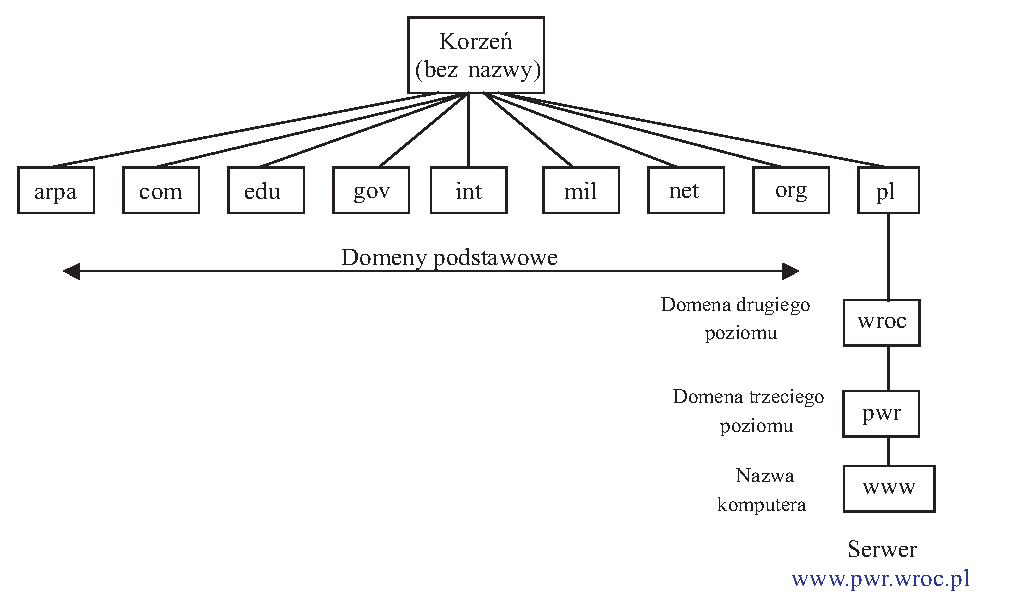
\includegraphics[width=5in]{./rysunki/struktura_dns.eps}
\caption{Hierarchiczna struktura DNS}
\label{dns}
\end{figure}
																
Domeny arpa, com, edu, gov, int, mil, net, org i domeny państwowe takie jak pl nazywamy domenami podstawowymi. 
Obejmują one następujące komputery: arpa -- sieć ARPANET; com -- organizacje komercyjne; edu -- instytucje edukacyjne; 
gov -- organizacje rządowe; int -- organizacje międzynarodowe; mil -- armia USA; net -- sieci; org -- pozostałe 
organizacje. Organizacje rządowe z krajów innych niż USA grupowane miały być w dwuliterowych domenach państwowych
np. ae -- Zjednoczone Emiraty Arabskie; pl -- Polska; zw -- Zimbabwe. Obecnie podział ten nie jest ściśle 
przestrzegany, wiele organizacji komercyjnych rejestruje się w domenie podstawowej (np. empik.com), inne stosują 
podział w ramach domen państwowych (np. creamsoft.com.pl). spotyka się również nazwy w ogóle nie mieszczące się 
w opisanym schemacie np. www.rmf.fm.

Obszarem nazywamy oddzielnie administrowaną część drzewa DNS. Typowym obszarem jest domena drugiego lub 
trzeciego poziomu  np. netscape.com lub pwr.wroc.pl. Jeśli w domenie zarejestrowanych jest wiele komputerów 
zwykle (dla zwiększenia efektywności działania DNS) dzieli się ją na kilka obszarów.

W każdym obszarze musi znajdować się podstawowy serwer DNS, który w specjalnym zestawie plików przechowuje 
odwzorowania wszystkich nazw komputerów z danego obszaru w ich adresy IP. Drugoplanowe serwery DNS informacje o 
odwzorowaniach uzyskują z serwera podstawowego korzystając z połączenia TCP o numerze portu 53. Serwery 
drugoplanowe przechowują (na zasadzie pamięci cache dla klientów, którzy zwracają się do nich z zapytaniami) 
odwzorowania obejmujące tylko część obszaru i odwzorowania o które klienci najczęściej pytają. W stałych 
odstępach czasu (typowo co 3 godziny) serwery drugoplanowe DNS uaktualniają swe tablice odpytując serwer 
podstawowy. Odwzorowanie nazwy spoza obszaru nie musi być znane ani serwerowi podstawowemu, ani drugoplanowemu, 
chyba że przechowywane jest w pamięci cache (jest często poszukiwane). Jeśli serwer podstawowy nie zna żądanego 
odwzorowania musi się zwrócić z zapytaniem (z wykorzystaniem portu 53 TCP) do jednego z serwerów głównych DNS 
(w 1993 roku było ich w Internecie 8), których obowiązkiem jest wskazanie serwera DNS będącego w stanie zwrócić 
poprawne odwzorowanie.

Proces odpowiedzialny za odwzorowanie nazw po stronie klienta nazywamy rezolwerem lub przelicznikiem nazw. 
Zwykle jest on zintegrowany z aplikacją (np. przeglądarką WWW) i na zasadzie pamięci cache przechowuje lokalnie 
pewną ilość odwzorowań. Jeśli wywoływana przez użytkownika nazwa nie jest znana lokalnie rezolwer korzystając z 
portu UDP 53 wysyła zapytanie do najbliższego drugoplanowego serwera DNS. Jeśli odpowiedź nie przekracza 512 
bajtów zwracana jest w postaci datagramu UDP, w przeciwnym wypadku jako datagram UDP wysyłane jest pierwsze 512 
bajtów i w nagłówku DNS ustawiana jest flaga informująca o tym fakcie. Zazwyczaj rezolwer ponawia wtedy 
zapytanie korzystając z portu 53 TCP, co umożliwia przesłanie pełnej odpowiedzi w jednym segmencie TCP. Rezolwer 
może wysłać dwa typy zapytań: zapytanie rekurencyjne umożliwia serwerowi DNS ,,konsultacje'' z serwerami wyższego 
rzędu przed zwróceniem odpowiedzi; zapytanie iteracyjne wymaga od niego natychmiastowej odpowiedzi, która jeśli 
dany serwer nie zna odwzorowania, musi mieć postać adresu IP serwera DNS będącego (wedle ,,wiedzy'' zapytanego 
serwera DNS) w stanie udzielić poprawnej odpowiedzi. Ze wskazanym serwerem DNS resolwer komunikuje się 
bezpośrednio. Ponieważ istnieje możliwość, że  nieprawidłowe zapytanie rekurencyjne nieskończenie będzie krążyć 
pomiędzy serwerami DNS w nagłówku DNS zdefiniowano pole ograniczające liczbę rekurencji. Wartość tego pola 
zmniejszana jest o jeden przez każdy serwer DNS, który przetwarza zapytanie. Zapytanie z zerową wartością tego 
pola jest odrzucane i serwer komunikuje błąd. W takim wypadku rezolwer może użyć zapytania iteracyjnego, ponowić 
zapytanie rekurencyjne ze zwiększoną wartością pola ograniczającego rekurencje lub zgłosić użytkownikowi błąd 
DNS. Rysunki \ref{rekurencyjne} i \ref{iteracyjne} przedstawiają obsługę obydwu typów zapytań \cite{barylo3}.
\begin{figure}[h]
\centering
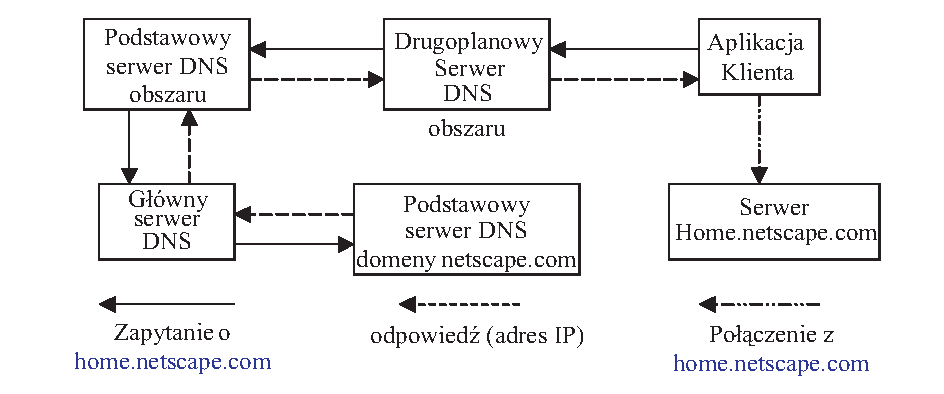
\includegraphics[width=4in]{./rysunki/zapytanie_rekurencyjne.eps}
\caption{Obsługa zapytania rekurencyjnego}
\label{rekurencyjne}
\end{figure}

\begin{figure}[h]
\centering
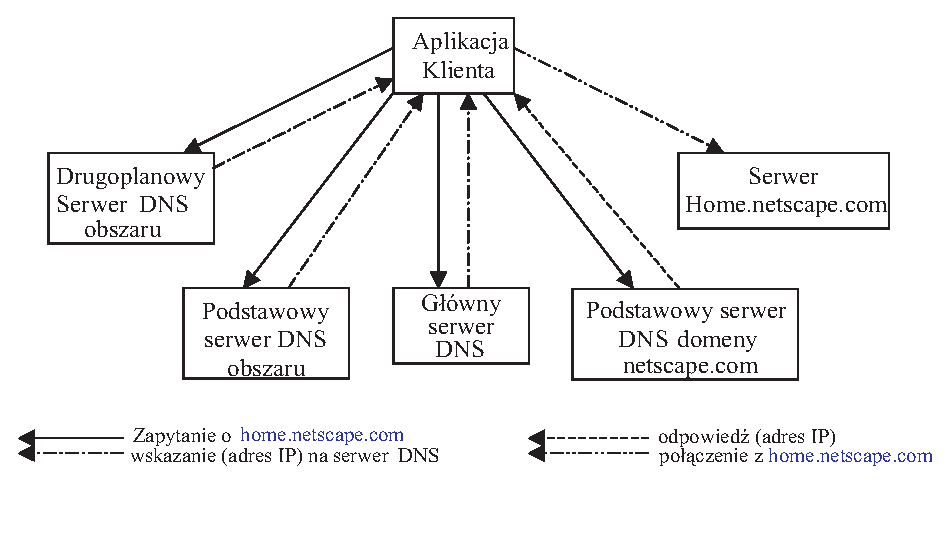
\includegraphics[width=4in]{./rysunki/zapytanie_iteracyjne.eps}
\caption{Obsługa zapytania iteracyjnego}
\label{iteracyjne}
\end{figure}

Powyższe rysunki przedstawiają ,,najgorszy'' przypadek, gdy adres IP serwera www.netscape.com znany jest dopiero 
przez podstawowy serwer DNS domeny (obszaru) netscape.com. W rzeczywistości istnieje duże prawdopodobieństwo, że 
odwzorowanie nazwy przechowywane jest przez pamięć cache jednego z bliższych klientowi serwerów.
Informacje o wzajemnych odwzorowaniach nazw w adresy IP serwery DNS przechowują w postaci rekordów zasobów 
DNS--DNS RR (ang. \emph{DNS Resource Record}). Rekordy te przesyłane są do aplikacji klienta jako odpowiedź na 
zapytanie. Pojedynczy DNS RR ma przedstawioną na rys. \ref{dns_rr} strukturę \cite{barylo3}.
\begin{figure}[h]
\centering
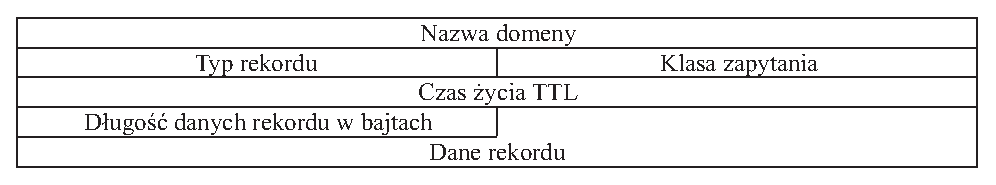
\includegraphics[width=5in]{./rysunki/format_dns_rr.eps}
\caption{Format DNS RR}
\label{dns_rr}
\end{figure}

Pole Nazwa domeny określa domenę do której odnoszą się dane rekordu. Pole Typ określa rodzaj danych np. czy 
rekord przechowuje odwzorowanie nazwy w adres IP, adresu w nazwę, czy tylko dodatkowe informacje o hoście. Pole 
Klasa ma zwykle wartość 1, co oznacza internetowy adres IP (niektóre serwery DNS udostępniają również adresy 
należące do innych protokołów np. IPX/SPX). Pole Czas życia TTL jest liczbą sekund określającą maksymalny czas 
przechowywania rekordu w pamięci cache rezolwera, niestety wiele aplikacji ignoruje tę wartość.

\section{Protokół HTTP}

W tym rozdziale 
szczegółowo omówiona jest specyfikacja protokołu HTTP oraz te właściwości protokołu, które rzutują na wydajność WWW.

\subsection{Specyfikacja HTTP}
 
Protokół HTTP (ang. \emph{HyperText Transfer Protocol}) jest prostym protokołem warstw górnych służącym do przesyłania 
dokumentów hipertekstowych w sieciach opartych o protokoły TCP/IP. W warstwie sieciowej HTTP korzysta z TCP i 
portu o numerze 80 \cite{barylo4}. 

Jak wspomniano dokument hipertekstowy zawierać może obok tekstu również grafikę, animacje, dźwięki oraz 
odsyłacze do innych dokumentów hipertekstowych, które mogą znajdować się na innych serwerach WWW, w konsekwencji 
często aby skompletować cały dokument przeglądarka WWW musi otworzyć wiele połączeń z kilkoma serwerami WWW.

HTTP wykonuje tylko przesyłanie plików składających się na dokument hipertekstowy. Jest to zazwyczaj plik 
będący opisem dokumentu w języku HTML, który zawiera tekst, informację o rozmieszczeniu elementów dokumentu oraz 
pliki będące reprezentacją takich elementów dokumentu jak grafika czy dźwięk. Ponieważ HTTP nie rozróżnia typów 
transmitowanych plików aplikacja serwera WWW jest dość prosta w porównaniu do aplikacji przeglądarki, która musi 
zinterpretować treść pliku HTML i odpowiednio rozmieścić na ekranie elementy dokumentu.

Istnieją dwa rodzaje komunikatów wymienianych pomiędzy klientem a serwerem HTTP: żądania i odpowiedzi. 
Format żądania HTTP ma następujący format:\\
	
	Linia--żądanie\\
	Nagłówki (0 lub więcej)\\
	<Linia pusta>\\
	Korpus (tylko dla żądania POST) \\

Format linii--żądania jest natomiast taki:\\
	
Dostępne są trzy różne żądania HTTP:
\begin{itemize}
\item żądanie GET, które zwraca dowolną informację (dokument) określoną przez następujący po nim URL;
\item żądanie HEAD, które zwraca tylko nagłówek wskazanego dokumentu, ten typ żądania wykorzystywany jest do sprawdzania 
odsyłaczy pod kątem aktualności lub dostępności;
\item żądanie POST używane do przesyłania danych od klienta do serwera np. przesyłania zawartości formularzy wypełnianych 
interakcyjnie przez użytkownika. Jest to jedyne żądanie wraz z którym przesyłany jest korpus komunikatu.
\end{itemize}

Format odpowiedzi HTTP jest następujący:\\

	Linia--stanu\\
	Nagłówki (0 lub więcej)\\
	<Linia pusta>\\
	Korpus\\

Format linii--stanu (status--line) ma następujący format:\\

	Wersja--HTTP kod--odpowiedzi fraza--odpowiedzi.\\

HTTP definiuje 17 różnych nagłówków, które dzielimy na 3 rodzaje: nagłówki używane z żądaniami, nagłówki używane 
z odpowiedziami, nagłówki określające korpus (przesyłane dane). Niektóre nagłówki mogą być używane zarówno z 
żądaniami jak i odpowiedziami (np. nagłówek DATE). Przykładowym nagłówkiem występującym z żądaniem jest nagłówek 
IF-MODIFIED-SINCE, który wraz z następującym po nim nagłówkiem DATE stanowi element tzw. warunkowego żądania 
GET. URL występujący w takim żądaniu jest otwierany tylko w przypadku jeśli był zmodyfikowany po wymienionej w 
żądaniu dacie. Jednym z nagłówków używanym z odpowiedziami jest LOCATION. Jego korpus stanowi nowy URL 
dokumentu, którego dotyczyło poprzednie zapytanie. Przykładem nagłówka określającego korpus jest LAST-MODIFIED. 
Następuje po nim nagłówek DATE, który podaje datę ostatniej modyfikacji dokumentu.
\begin{figure}[h]
\centering
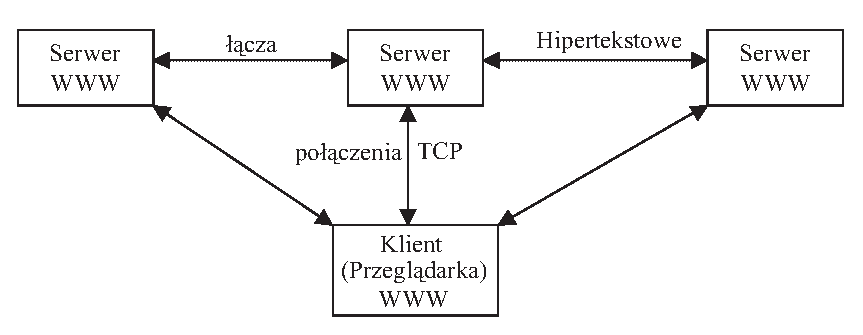
\includegraphics[width=5in]{./rysunki/polaczenia_w_sieci_www.eps}
\caption{Schemat połączeń w sieci WWW}
\label{polaczenia_www}
\end{figure}

Pierwsza linia odpowiedzi serwera nazywana jest linią stanu. Rozpoczyna ją określenie wersji HTTP, następnie 
podana jest trzycyfrowa liczba określająca kod odpowiedzi, a na końcu czytelne dla użytkownika wyrażenie. 
Poniższa tabela przedstawia znaczenie poszczególnych kodów odpowiedzi.

Starsze specyfikacje protokołu (HTTP 0.9 i HTTP 1.0) używały osobnego połączenia TCP do pobrania każdego 
elementu (pliku) wchodzącego w skład dokumentu. Najnowsza wersja HTTP 1.1 umożliwia stosowanie stałego, 
podzielonego na sesje połączenia TCP do pobrania całego dokumentu.

Poniżej omówiono istotne ze względu na wydajność WWW cechy protokołu HTTP.

\subsection{Właściwości ruchu generowanego przez HTTP, a wydajność WWW}

W okresie od stycznia 1994 do kwietnia 1995 udział komunikatów HTTP wśród wszystkich pakietów przesyłanych 
w szkieletowej sieci NSFNET wzrósł z 3\% do 36\% i wartość ta wykazywała stałą tendencję wzrostową. 

Badania prowadzone w USA wykazały niezależną od stopnia obciążenia serwera proporcję pomiędzy 
poszczególnymi typami żądań klienta. Żądania typu GET stanowią ok. 99\% ogółu komunikatów przetwarzanych przez 
serwer. 0,85\% komunikatów to żądania typu HEAD. Pozostałe 0,15\% stanowią żądania POST. 

Jeśli chodzi o odpowiedzi to 78\% do 92\% stanowią odpowiedzi typu 20x (odpowiedzi typu ,,sukces''). Odpowiedź typu 
304 obejmują 4\% do 14\% wysyłanych przez serwer komunikatów. Łącznie odpowiedzi typu 20x i 304 stanowią 92\% do 
97\% ogółu odpowiedzi. W przypadku pozostałych typów odpowiedzi różnice są już znaczne w zależności od rodzaju 
informacji na serwerze i jego popularności. Np. odpowiedzi 301 i 302 mogą mieć 0,3\% udział w odpowiedziach 
popularnego serwera publikującego informacje naukowe NCSA (ang. \emph{National Center for Supercomputer Applications}) 
do nawet 4,2\% w przypadku niewielkiego serwera uniwersyteckiego w Calgary. Odpowiedzi typu 40x i 50x stanowią 
zwykle od 1\% do 4\%. 

Typowo ilość danych przesyłanych w połączeniu HTTP jest niewielka. Żądania klienta nie przekraczają kilkuset 
bajtów, a pojedyncza odpowiedź serwera rzadko kiedy przekracza 10 kB.

Ciekawych informacji dostarczyć może analiza pomiaru czasu RTT (ang. \emph{Round Trip Time}), czyli łącznego czasu 
wymiany pakietu na drodze serwer -- klient -- serwer. Wartość ta jest używana przez TCP do wyznaczenia czasu 
retransmisji segmentu w przypadku braku potwierdzenia odbioru. Przybliżenie tego czasu można uzyskać dokonując 
pomiaru czasu trwania fazy zamykania połączenia TCP. Przytoczone tu wyniki otrzymano mierząc ten czas dla 19 
tyś. połączeń wykonanych przez 810 różnych klientów na terenie USA. Najmniejsza wartość wyniosła 0 sekund dla 
hosta lokalnego a największa 12,3 sekundy. Wartość średnia była równa 0,445 sekundy a mediana 0,187 sekundy. 
Wyniki te są zadziwiające jeśli wziąć pod uwagę, że teoretyczny RTT pomiędzy wschodnim i zachodnim wybrzeżem USA 
wynosi 0,06 sekundy. Odpowiedzialność za ten fakt ponosić może znaczna ilość klientów podłączonych poprzez modem 
(najszybszy nawet modem wprowadza ok. 0.2 sekundy opóźnienia do każdego pojedynczego pomiaru wartości RTT). 

Cechą bardzo niekorzystnie wpływającą na wydajność HTTP w jego starszych wersjach była konieczność otwierania 
osobnego połączenia TCP dla każdego elementu dokumentu. Wiele zależało tutaj od konstrukcji przeglądarki. Jeśli 
nie otwierała ona połączeń równoczesnych to pobranie całego dokumentu wydłużało się o czas konieczny na kolejne 
nawiązywanie i zamykanie połączeń. Jeśli z drugiej strony przeglądarka ,,agresywnie'' otwierała zbyt wiele 
połączeń równoczesnych, to barierą stawała się przepustowość połączenia z Internetem i wielkość MSS oferowana 
przez serwer. Znany jest przykład przeglądarki NCSA Mosaic, która potrafiła otworzyć kilkanaście równoczesnych 
połączeń TCP dla pobrania pojedynczego dokumentu, powodując tym zarówno zatory w sieci lokalnej jak i 
niepotrzebne obciążenie serwera. 

Otwieranie zbyt wielu połączeń równoczesnych nie przynosi spodziewanych korzyści. Podstawowym 
problemem wydajności HTTP wydaje się być niedopasowanie protokołu TCP -- zorientowanego na przesyłanie strumienia 
bajtów i usługi WWW zorientowanej na przesyłanie wyodrębnionych komunikatów. Należy pamiętać że HTTP, który jest 
w rzeczywistości protokołem przesyłania plików, miał w swych założeniach zapewniać wydajność większą niż 
protokół FTP. Chciano uzyskać to eliminując występujące w FTP dodatkowe połączenie sterujące (port 21) i 
konieczność nawiązywania połączenia TCP na dwóch portach. 

Niestety TCP wymaga zestawienia połączenia przed faktycznym rozpoczęciem transmisji. Wprowadza to opóźnienie o 
wartości ok. 1 RTT przed przesłaniem pliku. Dodatkowo w starszych wersjach HTTP pobranie dokumentu wymagało 
otwieranie nowego połączenia TCP dla każdego pliku składowego, co oznacza, że należało zamykać połączenia przez 
które wysłano wcześniejsze elementy dokumentu. Każdorazowe zamykanie i otwieranie połączeń wprowadza opóźnienie 
rzędu 3RTT dla każdego pliku składowego. HTTP 1.1 używa stałego łącza TCP dla dokumentu, co zredukowało 
opóźnienie przed rozpoczęciem transferu kolejnego elementu dokumentu do 1RTT. Dodatkowo HTTP 1.1 umożliwia 
wysyłanie żądań potokowych tzn. wysyłanie żądań o kolejne pliki przed rozpoczęciem odbierania poprzednio 
żądanych elementów dokumentu. Niestety w przypadku plików dynamicznych np. plików wynikowych skryptu CGI potok 
taki jest wstrzymywany. 